\documentclass[SDSUThesis.tex]{subfiles} 
\begin{document}


\section{A SOFTWARE DEVELOPMENT ORGANIZATION (SDO)}
A \textit{Software Development Organization} is any organization or subset of an organization that is responsible
for the creation, deployment, and maintenance of software.  Many times a software development organization
is a company that produces software.  Other times, a software development organization is contained
within the Information Technology department of a larger organization. Some of the job roles
with an SDO are: software engineer, system administrator, software quality analyst,
programmer, database administrator, and documentation specialist.


\subsection{WHAT IS SOFTWARE?}
Numerous definitions can be found for the term \textit{software}.
Software is more than just computer programs. According to Ian Sommerville \cite{Sommerville2001}, 
"Software is not just the programs but also all associated documentation and configuration data which is needed to make these programs operate correctly."
This is the definition used for the remainder of this work.


\subsection{THE SOFTWARE DEVELOPMENT LIFECYCLE}
    For this question, I choose to rewrite that section of the proposal.  This was
    my favorite question. It forced me to go look back into the history of
    software development. 
    
    The discipline of software engineering has created a workflow for developing
    software.  
    This workflow is called the \textit{Software Development Life Cycle (SDLC)}.
    SDLC can be defined as \cite{Ruparelia2010}:
    \begin{quote}
     [...] a conceptual framework or process that considers the structure of the stages
     involved in the development of an application from its initial feasibility study
     through to its deployment in the field and maintenance.
    \end{quote}
    While the SDLC states what needs to be done, there are numerous models 
    that formalize exactly how to perform the SDLC.  The models contain
    steps that are commonly referred to as a phases. A few of the popular
    models are described below.
    
    
    \subsubsection{WATERFALL}
        The waterfall model is the oldest and most influential of the SDLC models. 
        It was first presented at a Navy Mathematical Computing Advisory Panel in 1956
        by Herb Benington \cite{Benington1987}. Figure \ref{fig:benington} shows
        the model Benington outlined for producing large software systems.  
        In 1970, Benington's model was modified by Royce \cite{Royce1987}.  Royce
        produced an updated version of the diagram seen in Figure \ref{fig:royce}
        which provides some loops to go back to a previous phase in the workflow.
    
        \begin{figure}
            \centering
            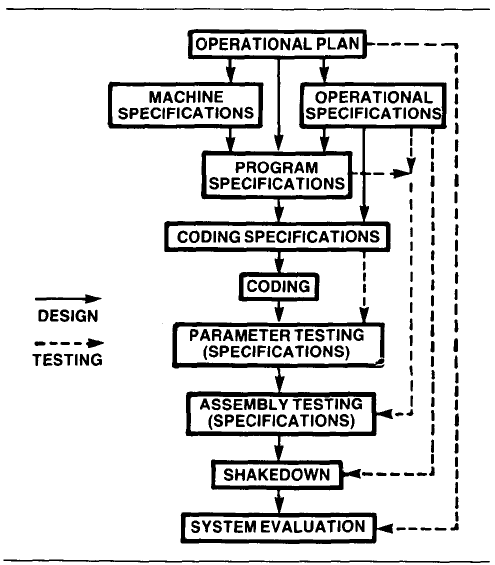
\includegraphics[scale=.5]{images/benington_waterfall.PNG}
            \caption[Benington's original diagram for producing large software systems]
                    {Benington's original diagram for producing large software 
                        systems, adapted from \cite{Benington1987}}
            \label{fig:benington}
        \end{figure}%
        \begin{figure}
            \centering
            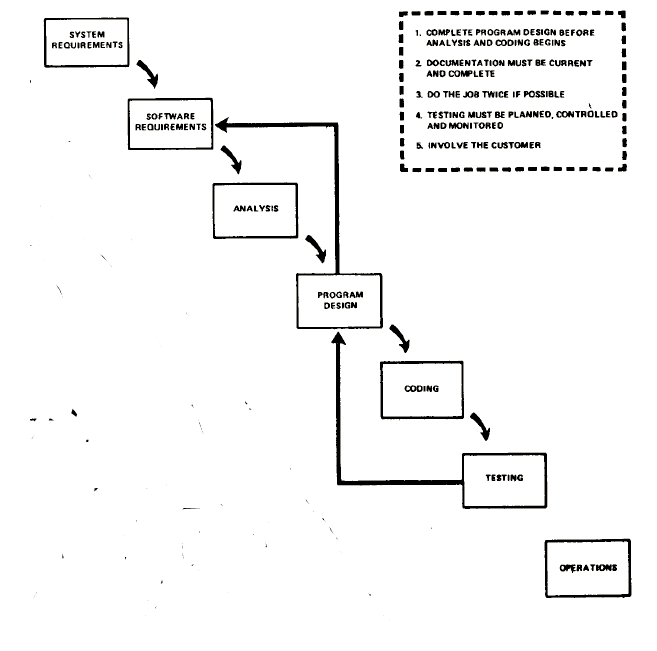
\includegraphics[scale=.5]{images/royce_waterfall.PNG}
            \caption[Royce's version of the waterfall model]
                {Royce's version of the waterfall model for producing software 
                        systems, adapted from \cite{Royce1987}}
            \label{fig:royce}
        \end{figure}
        
        The modern version of the waterfall model specifies that each phase needs 
        to be entirely completed before moving
        onto the next phase.  Some small amount of overlap is permitted and looping 
        occurs but both actions are discouraged and should be limited.  
        A modern diagram of the waterfall model can be seen in Figure \ref{fig:waterfall}.
        \begin{figure}[here]
            \centering
            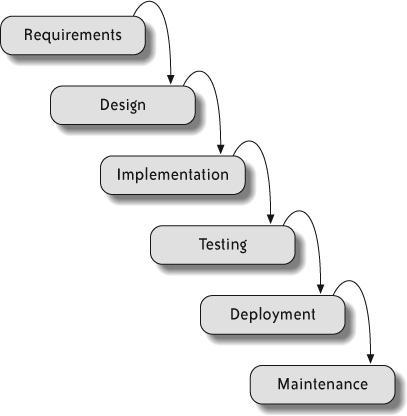
\includegraphics[scale=.6]{images/waterfall.png}
            \caption[Modern Waterfall]
                {Modern Waterfall Diagram, adapted from \cite{Hibbs2009} }
            \label{fig:waterfall}
        \end{figure}
        
        Waterfall has some excellent features such as: simple to understand,
        easy to plan, and well-defined phases. However, waterfall lacks
        the flexibility required of many software systems built today
        \cite{Maheshwari2012}.  Due to the fact the phases are so sequential,
        it makes changes during the life cycle difficult and expensive if 
        not impossible. Therefore, other models of SDLC have been created
        to address the lack of flexibility of the waterfall model. Notice,
        the other models are  adaptations of waterfall.
    
    
    \subsubsection{SPIRAL}
        
        The spiral model for software development was presented by Boehm in 1986
        \cite{Boehm1986, Boehm1988}. 
        The goal of the spiral mode of software development is very risk-driven.
        A software project will start with many small and quick iterations. 
        Each iteration will cover the following 4 basic steps. 
        \begin{enumerate}
            \item Determine Objectives
            \item Identify Risks
            \item Develop and Test
            \item Plan Next Iteration
        \end{enumerate}
        This model allows software to be built over a series of iterations
        without risking too much time or effort in any single iteration.
        Sprial requires a very adaptive management approach
        as well as flexibility of the key stakeholders \cite{Ruparelia2010}.
        It can also be difficult to identify risks that will occur in future
        iterations.
        Figure \ref{fig:spiral} provides a bit more detail on the iterations
        and the overall process. 
        \begin{figure}[here]
            \centering
            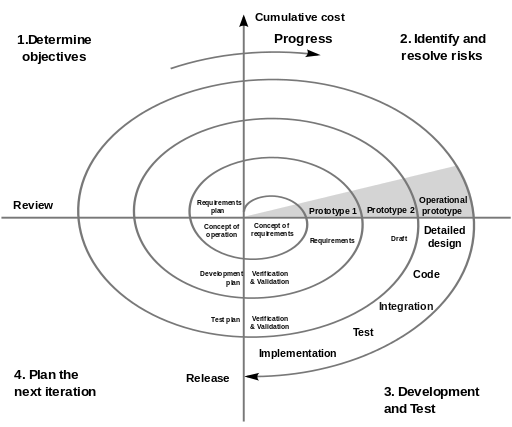
\includegraphics[scale=.5]{images/spiral_model.png}
            \caption[Spiral SDLC Model]{Spiral SDLC Model \cite{Boehm2000} }
            \label{fig:spiral}
        \end{figure}
        
        
    \subsubsection{AGILE}
        Agile software development has arisen due to the inability
        of the waterfall and other models to adjust to changes during the 
        development cycle.  
        Agile software development is a group of SDLC models that operate
        under the influence of the following four key principles \cite{Beck2001}.
        \begin{enumerate}
            \item Individuals and interactions over processes and tools
            \item Working software over comprehensive documentation
            \item Customer collaboration over contract negotiation
            \item Responding to change over following a plan
        \end{enumerate}
        Agile does not specify an implementation, but
        some specific models of agile SDLC are:
        eXtreme Programming, Scrum, Lean, Kanban and others 
        \cite{Moniruzzaman2013, Hibbs2009}.  Agile models 
        are very popular in many of today's software development
        organizations because the models work well for dynamic
        quickly changing applications such as web-based applications.
        
        
    \subsubsection{SDLC COMMONALITIES}
        Even with the large number of SDLC models currently being used by different SDOs,
        there is still some commonalities among the models.  The 
        commonalities can be tied back to the steps of waterfall.  All of the models
        exhibit, to some degree, the following phases. The only major difference is 
        the scope, size, and duration of each phase.  For example, the spiral
        model spends less time in each phase.  The agile models produce less
        documentation and focus more on the Implemenation phase. Here are
        the common phases in nearly all SDLC models:
        \begin{description}
            \item[1. Requirements] \hfill \\ The first phase is involved 
                with defining what the software must do.  Each piece of 
                functionality is considered a requirement.  
            \item[2. Design] \hfill \\ Before writing any code, the 
                necessary infrastructure and involved software systems
                must be identified. This phase can serve as a roadmap for the 
                remaining phases. If done properly, this phase can greatly 
                help the later phases.
            \item[3. Implementation] \hfill \\ Often the only phase of the SDLC 
                that is measured, this is the phase where the actual computer
                code is written.
            \item[4. Testing] \hfill \\ This phase validates the expected 
                functionality.  Also, testing attempts to discover unexpected
                side affects of the software.
            \item[5. Deployment and Maintenance] \hfill \\ All software must 
                be correctly deployed and maintained.  This phase is the 
                most expensive and lengthy phase of the software
                development lifecycle.
        \end{description}
        
\subsection{WHAT IS SOFTWARE ENGINEERING?}
    \textit{Software Engineering} as a term dates back to the 
    1968 North Atlantic Treaty Organization (NATO) conference \cite{Tsui2013, Naur1969}. Over the 
    years many definitions have been provided.  IEEE provides a definition that encompasses many of the
    other definitions.  IEEE defines software engineering as, 
    ''The application of a systematic, disciplined, quantifiable approach to the development, operation, and maintenance of software''
    \cite{Ieee1990}.
    
    
    Software engineering has struggled to determine the correct projects to complete \cite{DeMarco2009}.
    Software projects are typically behind schedule and over budget. Organizations need a better
    technique to understand the past performance so they can better predict the future performance.

\subsection{TERMINOLOGY}

\begin{description}
    \item[SIT]   (Systems Integration Testing) - The initial step of testing
        after the development phase of the SDLC.  This is typically 
        performed by members of the SDO.  It is validation that all the
        software components function together as expected.
    \item[UAT]   (User Acceptance Testing) - The final step of testing
        when a select few members of the user group are invited to
        validate the software system. Once validation has occured for
        UAT, the software system is ready to proceed to production
    \item[PROD]  (Production) - The software has been released to the final audience.
    \item[defect] Whenever the output of software does not meet expectations.  It is important to mention that even though defects are typically 
            found in the computer code, a defect should not be isolated to just code.   A poorly written requirement or missed test cases can 
            both be considered a defect.  Other common names for a defect are: bug, error, fault, or ticket.
            
            ``
                A software defect is a bug or error that causes
                software to either stop operating or to produce
                invalid or unacceptable results.
            '' as quoted from
            \cite{Jones2009}.  Also in here is the 4 severity levels.  Also, current defect removal is only about 85\% and this value should be increased to about 95\%. 
\end{description}

%\subsection{Data-Driven Software Engineering}
%Data Driven Software Engineering not Data Driven Software Development

%Check these book \cite{Jones2009, Jones1996, Lee2003}. This might be similar
%to process mining \cite{vanderAalst2012}.  

\end{document}